\section{Sequential Monte Carlo}
\subsection{Overview}
The last chapter was motivated by validating the use of Bayesian methods for solving inverse problems. However, the solution of Bayesian filtering problems, given by the sequence of posterior measures, often does not have a closed form solution. This requires us to construct numerical estimates of the sequence of posterior measures.

The class of estimators we will be considering for this task are \textit{sampling estimators}. Such estimators are constructed by using a set of \textit{particles} representing weighted points of the parameter space $X$ in order to estimate the distribution of interest. A building block of such estimators is the following operator

\begin{definition}
  Let $\mathcal{P}(X)$ denote the set of probability measures on $X$. Let $M \in \mathbb{N}$, for any measure $\mu \in \mathcal{P}(X)$ we define $S^M\mu$ by

  \begin{equation*}
    S^M\mu = \frac1{M}\sum_{i=1}^M\delta_{U_i},
  \end{equation*}

  where $U_1, \ldots, U_M$ are i.i.d. random variables distributed according to $\mu$. From the randomness of the samples $U_1, \ldots, U_M$, it follows that $S^M\mu$ is a not a probability measure, but a random variable taking values in $\mathcal{P}(X)$. The operator $\mu \mapsto S^M\mu$ is called \textit{sampling operator}.
\end{definition}

The sampling operator is the simplest building block we will use in the construction of particle algorithms, we will denote it by
 
\begin{equation*}
  \mu^y \xrightarrow{\text{sample}} S^M\mu^y.
\end{equation*}

When only using this single building block, we obtain the \textit{Monte Carlo} estimate, or \textit{empirical measure}, of $\mu^y$. One can easily check that the Monte Carlo estimate is unbiased, and we will later prove that it has a variance of order $\mathcal{O}(M^{-1})$, regardless of the dimension of $X$. This algorithm alone can only be used in specific situations where direct sampling from the distribution of interest is possible. In Bayesian filtering however, the sequence of posterior distributions $\mu^y_t$ is  often too complex to be directly sampled from, and a simple Monte Carlo estimate cannot be constructed. This requires us to extend the Monte Carlo method to let us approximate non-trivial distributions as well. \textit{Sequential Monte Carlo} (SMC) is such a method.

The rest of the chapter will be structured as follows. In Section 3.2, we will present more building blocks for constructing estimation algorithms and show how we can use them to construct several popular algorithms. These iterations over the simple Monte Carlo estimate will then finally lead us to the SMC algorithm. In Section 3.3, we prove convergence properties of different algorithm blocks, and use these properties to show that the SMC algorithm provides a good estimate of each distribution of the sequence of filtering posterior distributions. We will conclude the chapter in Section 3.4 by presenting and analysing numerical solutions to the pendulum problem.

\subsection{Sequential Monte Carlo}

\paragraph{Importance sampling} An additional basic building block of SMC samplers is the \textit{Importance Sampling} (IS) method. The IS method can be used to estimate probability measures $\mu^y$ of the form of (\ref{bayes-rule}) for which the Radon-Nikodym derivative with respect to the prior $\mu_0$ is only known up to an unknown normalizing constant. To create an estimate, the IS method relies on using an \textit{importance distribution} $\nu$ from which we can easily generate samples. If $\mu^y \ll \nu \ll \mu_0$, then by the chain rule for Radon-Nikodym derivatives and substituting by (\ref{bayes-rule}), we have

\begin{align*}
  \frac{\d\mu^y}{\d\nu}(u)
  &= \frac{\d\mu^y}{\d\mu_0}(u)\left(\frac{\d\nu}{\d\mu_0}(u) \right)^{-1}\\
  &= \frac1{Z_y}\ell(u|y)\left(\frac{\d\nu}{\d\mu_0}(u) \right)^{-1}\\
  &=: w(u) / Z_y.
\end{align*}

Where $w$ is the \textit{importance weight} function. This gives us for any $\mu^y$-integrable function $f$ the following equality

\begin{equation*}
  \mu^y(f) =  \nu(w \cdot f) / Z_y,
\end{equation*}
\begin{equation*}
  Z_y = \nu(w).
\end{equation*}

These two equalities allow us to use a Monte Carlo estimate of $\nu$ to create an estimate of $\mu^y$. Given i.i.d. samples $V_1, \ldots, V_M$ distributed according to $\nu$, we consider the Monte Carlo estimate $S^M\nu$ to define the estimates

\begin{equation*}
  \hat Z_y = S^M\nu(w) = \frac1M\sum_{i=1}^M{w(V_i)},
\end{equation*}
\begin{equation*}
  \hat\mu^y(f) = \frac{S^M\nu(w \cdot f)}{\hat Z_y} = \frac1{M\hat Z_y}\sum_{i=1}^M{w(V_i)f(V_i)}
               = \sum_{i=1}^MW_if(V_i),
\end{equation*}

where $W_i$ are the \textit{normalized importance weights} given by
\begin{equation*}
  W_i = \frac{w(V_i)}{\sum_{i=1}^M{w(V_i)}}.
\end{equation*}

Before discussing properties of IS, we first give a slightly different formulation of the IS method to allow us using it as a building block for other algorithms. Expressing $\mu^y$ in terms of $\nu$ can be encapsulated in a non-linear \textit{reweighting operator} $L^w$ given by

\begin{equation*}
  (L^w\nu)(\d u) = \frac{w \cdot \nu(\d u)}{\nu(w)},
\end{equation*}

which, from the definition of $w$, gives us the equality $\mu^y = L^w\nu$. We can thus define a reweighting transition that can be used to construct algorithms as

\begin{equation*}
  \nu \trarrow{reweight} L^w\nu = \mu^y.
\end{equation*}

Having this new building block, we can combine the reweighting operator with the sampling operator and get

\begin{equation*}
  \nu \trarrow{sample} S^M\nu \trarrow{reweight} L^wS^M\nu. 
\end{equation*}

We can then verify that the IS algorithm, written as a composition of the two blocks presented, delivers the same result as before

\begin{equation*}
  (L^wS^M\nu)(f)
               = \frac{S^M\nu(w \cdot f)}{S^M\nu(w)}
               = \frac{\sum_{i=1}^Mw(V_i)f(V_i)}{\sum_{i=1}^Mw(V_i)}
               = \sum_{i=1}^MW_if(V_i) = \hat\mu^y(f).
\end{equation*}

This formulation is thus identical to the previous formulation. However, we will later see how this modular definition of algorithms makes it easier to extend them and study their properties.

The IS method provides an unbiased estimate for the normalizing constant $Z_y$ and a biased estimate for $\mu^y(f)$ with both bias and variance of order $\mathcal{O}(M^{-1})$ \note{ref needed}. However, while this method provides asymptotic convergence results, we are interested in the non asymptotic regime and the constants involved. In this situation were $M$ is fixed, the variance of the estimation is proportional to the variance of the importance weights \note{ref}. This means that the estimator is only good if the importance distribution is \textit{close enough} to the distribution we want to sample from. In practice, finding good importance distributions can be hard for non-standard target distributions, which makes it hard or impossible to directly use IS. Yet, this does not imply that ideas of IS should be completely discarded, and we now show how IS can be extended to sample filtering distributions.

Considering a sequence of distributions such as (\ref{phi-seq}), we can expect consecutive distributions to be approximately close to each other. This means that each distribution $\mu^y_{t-1}$ should be a good importance distribution to use importance sampling on the next distribution $\mu^y_t$. This gives us for each importance sampling step $t$ from $\mu^y_{t-1}$ to $\mu^y_t$ an importance weight function $w_{t-1}$ and a reweighting operator $L_{t-1} = L^{w_{t-1}}$. We can thus iterate reweighting steps to map the prior distribution to any arbitrary distribution of the sequence of posteriors giving $\mu^y_t = (L_{t-1} \circ \ldots \circ L_0) \mu_0$ and

\begin{equation*}
  \mu_0 \trarrow{reweight} L_0\mu_0 = \mu^y_1 \trarrow{reweight} \ldots\trarrow{reweight} L_{t-1}\mu^y_{t-1} = \mu^y_t.
\end{equation*}

Similar to the IS method, we can use this equality to create an algorithm by applying the sequence of operators to a Monte Carlo estimate of $\mu_0$, giving the algorithm

\begin{align*}
  \mu_0 \trarrow{sample} S^M\mu_0
  &\trarrow{reweight} L_0S^M\mu_0\\
  &\ \ \ \ldots\\
  &\trarrow{reweight} (L_{t-1} \circ \ldots \circ L_0)S^M\mu_0.
\end{align*}

We note that in the common case where the posterior distributions are induced by potentials $\Phi_t$ given by (\ref{gaussian-potential}), the importance weight $w_{t-1}$ is then given by

\begin{equation}\label{simple-weights}
  w_{t-1}(u) = \frac{l_t(u|y)}{l_{t-1}(u|y)} = \exp\left(\Phi_{t-1}(u;y) - \Phi_t(u;y)\right) = \exp(-\left|y_t - \G_t(y)\right|^2_\Gamma),
\end{equation}

this implies that the reweighting operator can be efficiently implemented by only requiring $M$ evaluations of the forward response operator.

While this appears to be a valid algorithm for estimating the sequence of distributions, it does not work. A simple counter-example would be to consider estimating a sequence of Gaussian distributions shifting away from $\mu_0$ as $t$ increases. Since the initial set of samples will, with high probability, be concentrated around the mean of $\mu_0$, as $t$ increases the distributions will shift away from where the samples are located. This will cause the weights of each particle to decrease as $t$ increases, which in turn will increase the variance of the estimate and make each estimate worse than the previous one.

\paragraph{Sequential Importance Sampling} To avoid this, we introduce an additional step after applying the reweighting operator to \textit{correct} the position of the samples by getting them closer to the target distribution. This should then result in a better importance distribution for the next step. To do this correction, we construct for each posterior distribution $\mu^y_t$ an ergodic Markov chain with stationary distribution $\mu^y_t$ characterized by its Markov kernel $K_t$ from which we know how to sample the next state given the current state, i.e. for every $u \in X$ we can sample from $K_t(u, \cdot)$. Since the Markov chain is ergodic, the limiting distribution of the Markov chain is equal to its stationary distribution $\mu^y_t$ regardless of the initial distribution \note{ref?}. Considering the operator induced by the Markov kernel $K_t$ given by

\begin{equation*}
  (K_t\mu)(f) = \mu(K_t(f)) = \int_X\int_X f(u) K_t(x, \d u) \mu(\d x),
\end{equation*}

the theorem stated in the previous sentence implies that applying the operator $K_t$ to any distribution will get it closer $\mu^y_t$, the stationary distribution of the Markov chain. This lets us define a new correction building block

\begin{equation*}
  \mu \trarrow{correct} K_t\mu.
\end{equation*}

We can thus replace each step of reweighting in the previous algorithm by the operator $\Psi_t = K_tL_{t-1}$, giving for every $\mu$

\begin{equation*}
  (\Psi_t \mu)(\d u) = (K_tL_{t-1}\mu)(\d u) = \frac{\mu(w_{t-1} \cdot K_t(\d u))}{\mu(w_{t-1})},
\end{equation*}

which in turn, for every $\mu^y_t$-integrable function $f$ gives

\begin{equation*}
  (\Psi_t \mu)(f) = \frac{\mu(w_{t-1} \cdot K_t)(f)}{\mu(w_{t-1})} = \frac1{\mu(w_{t-1})}\int_X\int_Xf(u)K_t(x, \d u)w_{t-1}(x)\mu(\d x).
\end{equation*}

We can then verify that the operator $\Psi_t$ maps $\mu^y_{t-1}$ to the distribution $\mu^y_t$ by using that $\mu^y_t$ is invariant under $K_t$

\begin{equation*}
  (\Psi_t\mu^y_{t-1})(\d u)
  = (K_tL_{t-1}\mu^y_{t-1})(\d u)
  = (K_t\mu^y_t)(\d u)
  = \mu^y_t(\d u),
\end{equation*}

which gives us the transitions from any posterior distribution $\mu_{t-1}^y$ to $\mu^y_t$ by

\begin{equation*}
  \mu^y_{t-1} \trarrow{reweight} L_{t-1}\mu^y_{t-1} \trarrow{correct} \Psi_t\mu^y_{t-1} = \mu^y_t.
\end{equation*}

As previously done, we can apply the sequence of operators to map $\mu_0$ to any posterior distribution of the sequence $\mu^y_t$ giving $\mu^y_t = (\Psi_t \circ \ldots \circ \Psi_1)\mu_0$ and

\begin{align*}
  \mu_0
  &\trarrow{reweight} L_0\mu_0 \trarrow{correct} \Psi_1\mu_0 = \mu^y_1\\
  &\ \ \ldots\\
  &\trarrow{reweight} L_{t-1}\mu^y_{t-1} \trarrow{correct} \Psi_t\mu^y_{t-1} = \mu^y_t.
\end{align*}

Transforming this into an algorithm by performing a step of sampling on $\mu_0$ before applying the sequence of operators $\Psi_t \circ \ldots \circ \Psi_1$ gives the \textit{Sequential Importance Sampling} (SIS) algorithm

\begin{align*}
  \mu_0 \trarrow{sample} S^M\mu_0
  &\trarrow{reweight} L_0S^M\mu_0 \trarrow{correct} \Psi_1S^M\mu_0\\
  &\ \ \ldots\\
  &\trarrow{reweight} L_{t-1}(\Psi_{t-1} \circ \ldots \circ \Psi_1)S^M\mu_0 \trarrow{correct} (\Psi_t \circ \ldots \circ \Psi_1)S^M\mu_0.
\end{align*}

It remains to discuss the contruction of the Markov Kernels $K_1, \ldots, K_T$. The optimal choice for each step $t$ is the Markov chains generating i.i.d. samples of the posterior distribution $\mu^y_t$. However, this choice requires us being able to sample from $\mu^y_t$, which is not possible otherwise we could just use a Monte Carlo approximation. Thankfully, much work has been put in designing Markov kernels with specific invariant distribution from which it is easy to sample.

\paragraph{Sequential Monte Carlo} We have defined with SIS an algorithm that incrementally updates a population of weighted independent samples to fit a sequence of distributions. However, even if the SIS algorithm tries to correct the position of the particles to match the sequence of posterior distributions, the transitions applied by the Markov kernels only guarantee convergence in the asymptotic regime with respect to the number of transitions and particles. Since we are clearly not in this regime, we need to measure the impact of the re-weighting  procedure on the quality of the Monte Carlo estimate given by these weighted particles.

If we consider a Monte Carlo estimate induced by $M$ i.i.d. random variables $Y_1, \ldots, Y_M$ of variance $\sigma^2$, the variance of the uniformly weighted sum of these variables would be equal to $\sigma^2/M$. If we instead consider a weighted sum of these variables, such as the one given by the IS and SIS algorithms of the form

\begin{equation}\label{sum-s}
  S = \frac{\sum_{i=1}^Mw_iY_i}{\sum_{i=1}^Mw_i},
\end{equation}

what would now be the variance of this sum? If each particle has an approximately equal importance weight, and thus equal participation in the estimate, we would have a variance close to the uniform case $\sigma^2/M$. We know this might not be the case and we want to measure the effective number of independent random variables $M_{eff}$ used in this sum, called the \textit{effective sample size} (ESS). We assume that $S$ was generated by summing $M_{eff}$ equally weighted i.i.d. samples and thus has a variance of $\sigma^2/M_{eff}$. This lets us solve for $M_{eff}$ by using the variance of the weighted sum $S$ given in (\ref{sum-s}). The resulting effective sample size is then

\begin{equation}\label{ess}
  M_{eff} = \frac{\left(\sum_{i=1}^Mw_i\right)^2}{\sum_{i=1}^Mw_i^2}.
\end{equation}

We can verify that this value is indeed bounded by the actual number of samples $M$

\begin{equation*}
  M_{eff} = M^2\frac{\left(\frac1M\sum_{i=1}^Mw_i\right)^2}{\sum_{i=1}^Mw_i^2} \le M^2 \frac{\frac1M\sum_{i=1}^Mw_i^2}{\sum_{i=1}^Mw_i^2} = M,
\end{equation*}

where the inequality is the weighted Jensen's inequality. This tells us that if the weights are too imbalanced, the effective size of our sample is going to be much smaller than the number of particles we have, which results in a Monte Carlo estimate of higher variance.

We thus are interested in modifying our algorithm to control the variance of the weights within our population, and thus keep the ESS over a certain level $M_{thresh}$ close to $M$. To achieve this, the Sequential Monte Carlo (SMC) algorithm controls the ESS after each step of reweighting and performs a step of \textit{resampling} if the ESS is too low. The resampling will reset the population by applying the sampling operator to the current estimate. This will reset every weight to $M^{-1}$ and discard with high probability the particles with lower weights. Specifically, the resampling step maps the current population estimate of the posterior distribution $\mu^y_t$ to a new population with uniform weights,

\begin{equation*}
  \sum_{i=1}^MW^i_t\delta_{U_i} \trarrow{resample} S^M\left(\sum_{i=1}^MW^i_t\delta_{U_i}\right) = \sum_{i=1}^M\frac1M\delta_{V_i},
\end{equation*}

where $V_i = U_j$ with probability $W^j_t$. This finally gives us the sequence of measures $\nu^M_0, \ldots, \nu^M_T$ created by the SMC algorithm to approximate the sequence of posterior measures $\mu_0, \ldots, \mu^y_T$

\begin{align*}
  \nu_0 &= S^M\mu_0\\
  \nu_{t+1}^M &= \begin{cases}
    \Psi_{t+1}\nu^M_t\text{\ \ \ \ \ \ \ \ if $M_{eff} > M_{thresh},$ }\\
    S^M\Psi_{t+1}\nu^M_t\text{\ \ \ \ otherwise. }
  \end{cases}
\end{align*}

The final form of the standard Sequential Monte Carlo algorithm is given in Algorithm \ref{smc-alg}. We now proceed to proving convergence properties of the SMC algorithm.

\begin{algorithm}[h]
  \label{smc-alg}
  \caption{Sequential Monte Carlo}
  \textit{(1) $\mu_0 \trarrow{sample} S^M\mu_0 = \nu^M_0$}\\
  Sample each $U^i_0$ from $\mu_0$ and
  set each weight to $W^i_0 = M^{-1}$. \\
  \;
  \For{$t = 1,\ldots,T$} {
    \textit{(2.1) $K_t\nu^M_{t-1}\trarrow{reweight} \Psi_t\nu^M_{t-1}$}\\
    Adjust weights $\hat W^i_t = w_t(U^i_{t-1})W^i_{t-1}$ and normalize them according to

    \begin{equation*}
      W^i_t = \hat W^i_t \Big/ \left(\sum_{j=1}^M\hat W_t^j\right).
    \end{equation*}
    
    \textit{(2.2) $\nu^M_{t-1} \trarrow{correct} K_t\nu^M_{t-1}$ }\\
    Sample each $U^i_t$ from $K_t(U^i_{t-1}, \cdot)$.\\
    \;
    \textit{(2.3) $\Psi_t\nu^M_{t-1} \trarrow{resample} \nu^M_t$}\\
    Compute $M_{eff}$ according to (\ref{ess}).\\
    \If{$M_{eff} < M_{thresh}$} {
      Sample each $U^i_t$ from $\Psi_t\nu^M_{t-1}$ and set each weight to $W^i_t = M^{-1}$.
    }
  }
\end{algorithm}



\subsection{Convergence of the SMC algorithm}

In this section, we will prove properties of the different building blocks used in the construction of the SMC algorithm and use them to prove convergence of the algorithm. Since the output of the SMC algorithm is not deterministic, but instead a sequence of random probability measures, we will show that each of these approximations converges weakly to the true probabilities in the number of particles $M$ used for the approximation.

We first define the following metric over the space of random probability measures

\begin{definition}
  For every $\mu$ and $\nu$ random variables with values in $\mathcal{P}(E)$, we define

  \begin{equation*}
    d(\mu, \nu) := \underset{|f|_\infty\le1}{\text{sup}} \sqrt{\expec{|\mu(f) - \nu(f)|^2}}.
  \end{equation*}

Then $d$ is a metric over the space of random measures on $X$. To lighten the notation in upcoming proofs, if $\mu \in \mathcal{P}(X)$ and $\nu$ is a random variable in $\mathcal{P}(X)$, we will write $d(\mu, \nu)$ to denote $d(\delta_\mu, \nu)$.
\end{definition}

Note that this metric bounds the variance of the unbiased estimate of an integral. Indeed, if we wish to estimate $\mu(f)$ by approximating $\mu$ using the unbiased estimate $\nu$ coming from a randomized algorithm, the variance of the estimate would be given by

\begin{equation*}
  \mathbb{V}\text{ar}(\nu(f)) = \expec{\left|\nu(f) - \expec{\nu(f)}\right|^2} = \expec{\left|\nu(f) - \mu(f)\right|^2} \le d(\nu, \mu)^2.
\end{equation*}

Hence, many of the results given in the coming lemma will not only show prove weak convergence of our approximations, but also bound the variance of the estimates as the number of particles increases.

The following lemma shows that it is enough to prove convergence in the metric $d$ to prove weak convergence of our estimates

\begin{lemma}
  Let $(\mu_n)_{n \in \mathbb{N}}$ be a sequence of random probability measures in $\mathcal{P}(X)$ and $\mu \in \mathcal{P}(X)$ such that $\underset{n \rightarrow \infty}{\text{lim}} d(\mu_n, \mu) = 0$, then the sequence $(\mu_n)_{n \in \mathbb{N}}$ converges weakly to $\delta_\mu$.
\end{lemma}
\begin{proof}
  Let $(\mu_n)_{n \in \mathbb{N}}$ be a sequence of random measures converging to $\delta_\mu$ in $d$. We recall that $(\mu_n)_{n \in \mathbb{N}}$ converges weakly to $\delta_\mu$ if and only if
  \begin{equation*}
    \underset{n \rightarrow \infty}{\text{lim}}\expec{\left|\mu_n(f) - \mu(f)\right|} = 0,
  \end{equation*}

  for every continuous and bounded function $f : X \rightarrow \mathbb{R}$. Let $f$ be such a function, we then have by Jensen's inequality

  \begin{equation*}
    \expec{\left|\mu_n(f) - \mu(f)\right|}  = \sqrt{\expec{\left|\mu_n(f) - \mu(f)\right|}^2} \le \sqrt{\expec{\left|\mu_n(f) - \mu(f)\right|^2}}
  \end{equation*}

  Since $f$ is continuous, it is also  measurable and by linearity of the integral and expectation we can assume without loss of generality that $|f|_\infty \le 1$. The proof is completed by bounding the right hand side of the equation by its supremum over all $|f|_\infty \le 1$

  \begin{equation*}
    \expec{\left|\mu_n(f) - \mu(f)\right|} \le \underset{|f|_\infty\le1}{\text{sup}} \sqrt{\expec{|\mu_n(f) - \mu(f)|^2}} = d(\mu_n, \mu) \overset{n \rightarrow \infty}{\longrightarrow} 0.
  \end{equation*}
\end{proof}

We start by showing that the sampling operator can approximate any probability measure to an arbitrary precision using enough samples.

\begin{lemma}\label{sampling-bound}
  The sampling operator satisfies

  \begin{equation*}
    \underset{\mu \in \mathcal{P}(X)}{\text{sup}}\ d(S^M\mu, \mu) \le \frac1{\sqrt{M}}
  \end{equation*}
\end{lemma}

\begin{proof}
  Let $\mu$ be an element of $\mathcal{P}(E)$ and $U_1, \ldots, U_M$ be i.i.d. random variables distributed according to $\mu$. For every measurable $f$ with $|f|_\infty \le 1$ we have 
  
  \begin{equation*}
    (S^M\mu)(f) - \mu(f) = \frac1{M}\sum_{i=1}^Mf(U_i) - \mu(f) = \frac1{M}\sum_{i=1}^Mf_i,
  \end{equation*}

  where $f_i = f(U_i) - \mu(f)$. This gives

  \begin{equation*}
    \left|(S^M\mu - \mu)(f)\right|^2
    = \left(\frac1{M}\sum_{i=1}^Mf_i\right)^2
    = \frac1{M^2}\sum_{i,j=1}^Mf_if_j.
  \end{equation*}

  Since we are interested in the expected value of this term, we now consider $\expec{f_if_j}$. For $i \neq j$, $f_i$ and $f_j$ are independent random variables, thus $\expec{f_if_j} = \expec{f_i}\expec{f_j}$, and since $U_i \sim \mu$, we have $\expec{f_i} = \expec{f(U_i)} - \mu(f) = 0$, giving $\expec{f_if_j} = 0$ for $i \neq j$. Furthermore, since $|f|_\infty \le 1$ we have

  \begin{equation*}
    \expec{f_i^2} = \mathbb{V}\text{ar}[f(U_i)] = \expec{f(U_i)^2} - \expec{f(U_i)}^2 \leq 1.
  \end{equation*}

  By linearity of the expected value, we then have for every $f$ with $|f|_\infty \le 1$

  \begin{equation*}
    \expec{\left|(S^M\mu)(f) - \mu(f)\right|^2} = \frac1{M^2}\sum_{i=1}^M\expec{f_i^2} \le \frac1{M}.
  \end{equation*}

  Taking the square root on both sides of the equation and the supremum over all such $f$ yields the desired result.
\end{proof}

Before proving the main result, we formalize the assumption that consecutive posterior distributions from a filtering problem should be close to each other.

\begin{assumption}\label{kappa-assumption}
  The importance weights $w_0, \ldots, w_{T-1}$ have the following property. There exists a $\kappa > 0$ such that for every $t \in \mathbb{N}$ and $u \in X$

  \begin{equation*}
    \kappa \leq w_t(u) \leq 1/\kappa.
  \end{equation*}
\end{assumption}

For convenience, we show that if the inverse problem is well-posed and the sequence of posterior distributions given by the potential functions (\ref{phi-seq}) do satisfy the previous assumption on any bounded parameter space $X$.

\begin{lemma}\label{easy-lemma}
  Assume that the potentials functions $\Phi_1, \ldots, \Phi_T$ are given by (\ref{phi-seq}), that the forward response operators $\G_1, \ldots, \G_T$ satisfy Assumptions \ref{assumption-fw} and that $X$ is bounded. Then, given some fix observation $y \in Y^T$, the importance weights $w_0, \ldots, w_T$ given in (\ref{simple-weights}) satisfy Assumption \ref{kappa-assumption}.
\end{lemma}

\begin{proof}
  We first show that $w_{t-1}(u)$ has an upper bound for each $t = 1, \ldots, T$ by

  \begin{equation*}
    w_{t-1}(u)
    = \frac{\ell_t(u|y)}{\ell_{t-1}(u|y)}
    = \exp\left(-\norm{y_t - \G_t(u)}_Y^2\right) \le 1
  \end{equation*}

  Then, using Assumption \ref{assumption-fw}(1), there exists an $M \in \mathbb{R}$ such that
  
  \begin{equation*}
    \norm{\G_t(u)}_Y^2 \le \exp(\norm{u}_X^2 + M).
  \end{equation*}

  If further $C = \underset{u \in X}{\sup} \norm{u}_X^2$, we have
  \begin{align*}
    w_{t-1}(u)
    &= \exp\left(-\norm{y_t - \G_t(u)}_Y^2\right)\\
    &\ge \exp\left(-\norm{y_t}_Y^2 - \norm{\G_t(u)}_Y^2\right)\\
    &\ge \exp\left(-\norm{y_t}_Y^2 - \exp(C+M)\right).
  \end{align*}

  The proof is complete by setting $\kappa = \min\{1, \exp\left(-\norm{y_t}_Y^2 - \exp(C+M)\right)\}$.
\end{proof}

We now show that the composition of reweighting and correction found in the SIS and SMC algorithm is Lipschitz continuous. This property is necessary to ensure that the asymptotic quality of the sampling approximation will not be lost by this additional step.

\begin{lemma} \label{seq-bound}
  Assume that the importance weights $w_0, \ldots, w_{T-1}$ satisfy Assumption \ref{kappa-assumption}. Then for any $t \in \mathbb{N}$ and $\mu, \nu \in \mathcal{P}(X)$,

  \begin{equation*}
    d(\Psi_t\mu, \Psi_t\nu) \leq \frac2{\kappa^2}d(\mu, \nu).
  \end{equation*}
\end{lemma}

\begin{proof}
  Let $f : X \rightarrow \mathbb{R}$ be a measurable function with $|f|_\infty \le 1$, we then have

  \begin{equation*}
    \begin{aligned}
      (\Psi_t\mu - \Psi_t\nu)(f)
      &= (K_tL_{t-1}\mu - K_tL_{t-1}\nu)(f) \\
      &= \frac{\mu(w_{t-1}K_t(f))}{\mu(w_{t-1})} - \frac{\nu(w_{t-1}K_t(f))}{\nu(w_{t-1})} \\
      &= \frac{\mu - \nu}{\mu(w_{t-1})}(w_{t-1}K_t(f)) + \frac{\nu(w_{t-1}K_t(f))}{\mu(w_{t-1})} - \frac{\nu(w_{t-1}K_t(f))}{\nu(w_{t-1})}\\
      &= \frac{\mu - \nu}{\mu(w_{t-1})}(w_{t-1}K_t(f)) + \nu(w_{t-1}K_t(f))\left(\frac1{\mu(w_{t-1})} - \frac1{\nu(w_{t-1})}\right)\\
      &= \frac{\mu - \nu}{\mu(w_{t-1})}(w_{t-1}K_t(f)) + \frac{ \nu(w_{t-1}K_t(f))}{\mu(w_{t-1})\nu(w_{t-1})}(\nu - \mu)(w_{t-1}).
    \end{aligned}
  \end{equation*}
  
  By Minkowski's inequality, we then have

  \begin{equation*}
    \begin{aligned}
      \sqrt{\expec{|(\Psi_t\mu - \Psi_t\nu)(f)|^2}}
      &\leq \expec{\left|\frac{\mu - \nu}{\mu(w_{t-1})}(w_{t-1}K_t(f))\right|^2}^{\frac12}\\
      &+ \expec{\left|\frac{ \nu(w_{t-1}K_t(f))}{\mu(w_{t-1})\nu(w_{t-1})}(\nu - \mu)(w_{t-1})\right|^2}^{\frac12}      .
    \end{aligned}
  \end{equation*}


  In the second term, since $\frac{\nu(w_{t-1}K_t(f))}{\nu(w_{t-1})} = (\Psi_t \nu)(f)$ and $|f|_\infty \le 1$, we have $\frac{\nu(w_{t-1}K_t(f))}{\nu(w_{t-1})} \le 1$. Further, since $w_{t-1}(u) \ge 1/\kappa$ for all $u$, it holds that $\mu(w_{t-1}) \ge \kappa$ and $1 / \mu(w_{t-1}) \le 1/\kappa$. From these two bounds, we obtain

  \begin{equation*}
    \begin{aligned}
      \sqrt{\expec{|(\Psi_t\mu - \Psi_t\nu)(f)|^2}}
      &\le \frac1\kappa\expec{|(\mu - \nu)(w_{t-1}K_t(f))|^2}^{\frac12}\\
      &+ \frac1\kappa\expec{|(\mu - \nu)(w_{t-1})|^2}^{\frac12}.
    \end{aligned}
  \end{equation*}


  Finally, using that $0 \le w_{t-1} \le 1/\kappa$, we have $|\kappa w_{t-1}|_\infty \le 1$ and similarly $[w_{t-1}K_t(f)](u) = \int_X f(y)w_{t-1}(u)K_t(u, \text{d}y) \leq |fw_{t-1}|_\infty K_t(X, u) \leq 1 / \kappa$, thus making $|\kappa w_{t-1}K_t(f)|_\infty \leq 1$. Bounding our expression by the supremum gives us 

  \begin{equation*}
    \sqrt{\expec{|(\Psi_t\mu - \Psi_t\nu)(f)|^2}} \le \frac2{\kappa^2}\underset{|g|_\infty \le 1}{\text{sup}} \sqrt{\expec{|\mu(g) - \nu(g)|^2}} =  \frac2{\kappa^2}d(\mu, \nu).
  \end{equation*}

  Since this result is valid for all $f$ with $|f|_\infty \le 1$, taking the supremum on the left hand side of the inequality yields the desired result.
\end{proof}

\begin{theorem}
  Assume that the importance weights $w_0, \ldots, w_{T-1}$ satisfy Assumption \ref{kappa-assumption} and consider the SMC algorithm with $M_{thresh} = M$. Then, for any $t \in \mathbb{N}$,

  \begin{equation*}
    d(\nu_t, \nu_t^M) \leq \frac1{\sqrt{M}}\sum_{j=0}^t\left(\frac2{\kappa^2}\right)^j.
  \end{equation*}
\end{theorem}

\begin{proof}
  For $t=0$, the result holds by direct application of Lemma \ref{sampling-bound}. For $t > 0$ we have using the triangle inequality, Lemmata \ref{sampling-bound} and \ref{seq-bound}, and using the induction hypothesis

  \begin{equation*}
    \begin{aligned}
      d(\nu_t, \nu_t^M)
      &= d(\Psi_t\nu_{t-1}, S^M\Psi_t\nu_{t-1}^M)\\
      &\le d(\Psi_t\nu_{t-1}, \Psi_t\nu_{t-1}^M) + d(\Psi_t\nu_{t-1}^M, S^M\Psi_t\nu_{t-1}^M)\\
      &\le \frac2{\kappa^2}d(\nu_{t-1}, \nu_{t-1}^M) + \frac1{\sqrt{M}}\\
      &\le \frac2{\kappa^2}\frac1{\sqrt{M}}\sum_{j=0}^{t-1}\left(\frac2{\kappa^2}\right)^j + \frac1{\sqrt{M}}\\
      &= \frac1{\sqrt{M}}\sum_{j=0}^t\left(\frac2{\kappa^2}\right)^j.
    \end{aligned}
  \end{equation*}
\end{proof}

This theorem shows that the SMC algorithm has an asymptotical variance $\mathcal{O}(d(\mu_t, \mu^M_t)^2) = \mathcal{O}(M^{-1})$. To conclude this section on the convergence analysis of the SMC algorithm, we first point that while the SMC algorithm is biased \note{ref}, the asymptotical magnitude of the bias is of order $\mathcal{O}(M^{-1})$. Since the mean square error (MSE) can be decomposed as $MSE = bias^2 + variance$, the mean square error of the SMC algorithm is dominated by the variance of the estimate, which is of $\mathcal{O}(M^{-1})$.

\subsection{Numerical solution to the pendulum problem}

In this section, we present and analyse the numerical solution of the filtering problem associated to the pendulum experiment. We start by showing that the pendulum filtering problem satisfy Assumption \ref{kappa-assumption} which implies that the SMC estimation of the sequence of posteriors converges. As a reference, we present the MCMC estimation solution of the Bayesian inverse problem associated to the pendulum problem. 

In the first experiment, we estimate the solution to the Bayesian inverse problem found by considering all the available data of the pendulum problem. We used the MCMC algorithm for $10,000$ steps and construct the Markov chain using Metropolis-Hasting kernel with Gaussian proposals of variance $0.1$. We have found that a burn-in period of $500$ steps was enough to reach equilibrium distribution. After $5$ runs of the algorithm, we find an mean estimate of $\expec{u|y} = 9.86 \pm \mathcal{O}(10^{-3})$ and a variance of $\mathcal{O}(10^{-6})$. This result is consistent with the unnormalized likelihoods presented in Figure \ref{uncertainty-posteriors}, and validate the theoretical results stated in Lemma \ref{sampling-bound}. A typical run of the algorithm is given in Figure \ref{mcmc-figure}.

\begin{figure}[t!]
  \label{mcmc-figure}
  \begin{minipage}{.43\textwidth}
    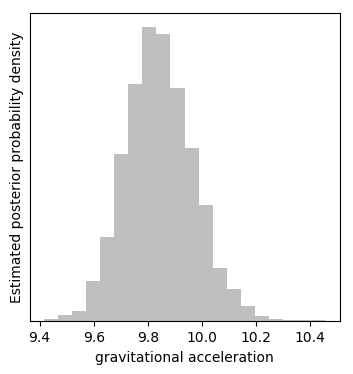
\includegraphics[width=\linewidth]{mcmc}
  \end{minipage}
  \begin{minipage}{.5\textwidth}
    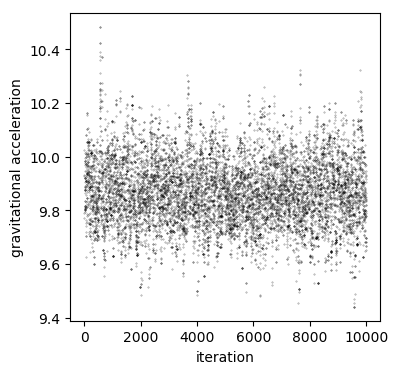
\includegraphics[width=0.97\linewidth]{mcmc-mixin}
  \end{minipage}
  \caption{Left: estimated posterior distribution using $M=10,000$ samples from the MCMC algorithm. Right: samples of the Markov chain for one run on the MCMC algorithm.}
\end{figure}

However, we are interested in approximating the sequence of filtering posterior distributions arising from the pendulum problem. In the following experiments, we use the sequence of importance weights given in (\ref{pendulum-weights}). Since we fulfill all assumptions stated in Lemma \ref{easy-lemma}, it also satisfies Assumption \ref{kappa-assumption} and the solution provided by the SIS and SMC algorithms weakly converge in $M$ to the true posteriors. In both algorithm, we use Metropolis-Hastings kernels with Gaussian proposals of variance $0.05$. 

In the second experiment, we illustrate why the step of resampling is crucial in the SMC algorithm. We run the SIS algorithm with $M=5,000$ particles and monitor the ESS as well as the importance weights over time. As expected, the experiment shows that the variance of the weights increase with both very large and very small weights, meaning that most of the probability mass of the particle estimate is contained in only a few estimate. This is also shown by the convergence of the ESS to a value of order $\mathcal{O}(1)$. These two results are shown in Figure \ref{sis-figure}.

Finally, we run a last experiment in which we run the SMC algorithm with $M_{thresh} = M/2$ for different values of $M$.

the code is running right now, missing plots are
\begin{itemize}
\item sequence of estimates for 5 MCMC updates
\item convergence of the mean/variance
\item comparison to MCMC and conclusion of the section
\end{itemize}

\begin{figure}[h]
  \label{sis-figure}
  \begin{minipage}{.5\textwidth}
    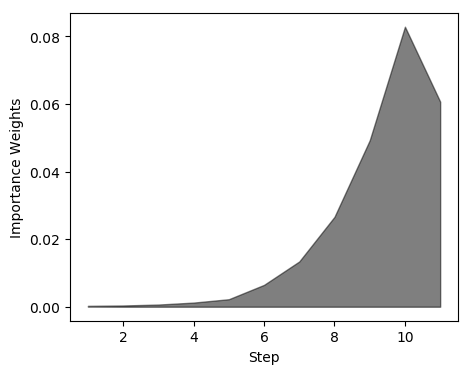
\includegraphics[width=\linewidth]{importance-weights-sis}
  \end{minipage}
  \begin{minipage}{.5\textwidth}
    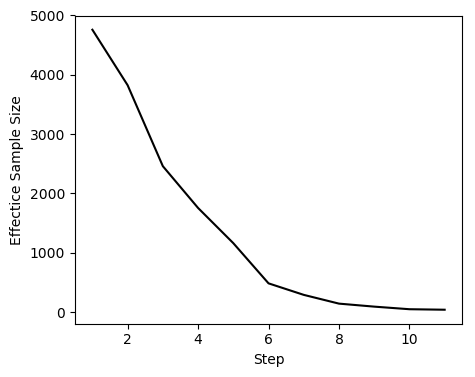
\includegraphics[width=0.97\linewidth]{ess-decay}
  \end{minipage}
  \caption{Left: the evolution of the importance weights of the particle estiamtes. The upper and lower bounds of the shaded area represent the value of the largest and smaller importance weight of the population. We can see that close to the end, a single particle contain almost all mass of the estimated probability measure. Right: evolution of the ESS over time, we see that after half the total number of iterations, the ESS is already only almost 1. }
\end{figure}

%%% Local Variables:
%%% mode: latex
%%% TeX-master:"Thesis"
%%% End:
